\documentclass[12pt]{article}
\usepackage{sbc-template}
\usepackage{graphicx}
\usepackage{amsmath}
%\usepackage{subfigure}
%\usepackage{times,amsmath,epsfig}
%\usepackage{graphicx,url}
 \makeatletter
 \newif\if@restonecol
 \makeatother
 \let\algorithm\relax
 \let\endalgorithm\relax 
\usepackage[lined,algonl,ruled]{algorithm2e}
\usepackage{multirow}
\usepackage[brazil]{babel}
\usepackage[utf8]{inputenc}  

\sloppy

\title{TRABALHO PRÁTICO 2: \\ Montador}

\author{Pedro Lopes Miranda Junior}

\address{Departamento de Ciência da Computação -- Universidade Federal de Minas Gerais (UFMG)
\email{plmj@dcc.ufmg.br}
}

\begin{document}
\maketitle

\begin{resumo} 
Este trabalho constitui na implementação de um montador para a linguagem de
máquina da máquina virtual criada anteriormente.
\end{resumo}

\section{Introdução}
\label{introducao}
Ao longo do curso serão estudados diversos conceitos sobre liguagem de máquina.
Perante isso, serão dados diversos trabalhos que testarão alguns dos inúmeros
conceitos abordados.

Após a implementação de uma máquina virtual é necessário um montador que
traduza um programa de uma linguagem assembly para a linguagem de máquina
criada anteriormente.

O montador lê o assembly passado por parâmetro e gera um código,em linguagem de
máquina, com as instruções criadas anteriormente. Além das funções contidas na
máquina virtual criada temos ainda as funções WORD e END.
A primeira cria a partir de um label uma constante que pode ser chamada nas
operações que usam a memória. A segunda apenas indica o fim do programa.

O montador faz duas passagens sendo a primeira para decodificar a tabela de
símbolos e a segunda para gerar o arquivo em linguagem de máquina.

Ao todo o montador suporta 25 operações, sendo elas as mesmas da máquina
virtual, porém com adição de WORD e END.

\section{Solução Proposta}
\label{solucao_proposta}
Para solucionar o problema, foi criada uma estrutura de dados que chama
mounter (Montador) que contém a tabela de símbolos.

Já a tabela de símbolos guarda o nome e o valor apontado pela label.

\subsection{Algoritmos}

Foram implementadas algumas funções que auxiliam no funcionamento do montador, 
portanto todas as funções operam sobre o tipo mounter.

\newpage

\subsubsection{Funções}
\begin{algorithm}[h!]
\begin{footnotesize}
   \textbf{initialize;} \textit{Inicializa o montador} \\
   \textbf{verlabel;} \textit{Verifica a existencia de um possível label} \\
   \textbf{veroperators;} \textit{Verifica quantos operadores tem a operação} \\
   \textbf{comment;} \textit{Verifica e tira os comentários} \\
   \textbf{vertab;} \textit{Busca na tabela de símbolo} \\
   \textbf{verreg;} \textit{Verifica qual o registrador deverá ser escrito} \\
   \textbf{printtab;} \textit{Imprime as informações quando no modo verbose} \\
   \textbf{firststep;} \textit{Imprime as informações quando no modo verbose} \\
   \textbf{secondstep;} \textit{Imprime as informações quando no modo verbose} \\
\caption{Funções do montador}
\end{footnotesize}
\end{algorithm}


\section{Implementação}
\label{implementacao}
Na implementação do problema proposto foram tomadas várias decisões, dentre
elas criar um tipo de dados para o montador, dividir o código em funções
de modo que na função principal fique o menor conteúdo possível ajudando no
encapsulamento do código e em futuras manutenções e melhorias.

Foi decidido criar um tipo de dados para o montador pois esse tipo de
disposição facilita a adição futura de demais estruturas.
Além disso o acesso ao TAD é feito de maneira melhor estruturada e o
encapsulamento é melhor feito.

A divisão do código em funções ajuda no encapsulamento do TAD, e na melhor
modularização do mesmo.

\subsection{Código}
O código foi dividido em arquivos \textit{.c} e \textit{.h} que estão listados
abaixo

\subsubsection{Arquivos .c}
\begin{itemize}
\item \textbf{mounter.c:} Contém a função principal do montaodr;
\item \textbf{mounterdata.c:} Contém as funções do tipo mounter;
\end{itemize}

\subsubsection{Arquivos .h}

\begin{itemize}
\item \textbf{mounterdata.h:} Contém as definições das funções do tipo mounter
\end{itemize}

\subsection{Compilação}

O programas deve ser compilado através de um makefile, chamando
\textit{montador}
ou através do compilador GCC chamando:\\

\begin{footnotesize}
\begin{verbatim} gcc -Wall mounter.c mounterdata.c -o montador \end{verbatim}
\end{footnotesize}

\subsection{Execução}

Para a execução do programa deverão ser recebidos,impreterívelmente, 
o modo de saída - S ou V - dos dados, o nome do arquivo com o código assembly a ser
executado e o arquivo de saída.

O comando para execução do programa é da forma: \\

\begin{footnotesize}
\begin{verbatim} ./vm  <modo> <entrada> <saída> \end{verbatim}
\end{footnotesize}

\subsubsection{Formato da entrada}
O arquivo de entrada citado deverá ser um programa em linguagem assembly,
onde cada linha conterá uma instrução, como abaixo:

\begin{footnotesize}
\begin{verbatim}
LOAD RA M7
LOAD RD M0
LOAD RC M0
SUM: READ NUM1
LOAD RB NUM1
ADD RC RB 
LOAD RA M1
ADD RD RA
LOAD RA M7
COMP RA RD
BNZ SUM;
STORE NUM1 RC
WRITE NUM1
HALT
M7: WORD 7
M0: WORD 0
M1: WORD 1
NUM1: WORD 0
END
\end{verbatim}
\end{footnotesize}

\subsubsection{Formato da saída}
O programa imprimirá no arquivo de saída o código em linguagem de máquina.
Além disso, caso o programa esteja rodando no modo verbose - V -  a tabela de
símbolos será impressa na saída padrão do sistema.
Para o exemplo acima, em modo simples a impressão no arquivo de saída será:\\
\begin{footnotesize}
\begin{verbatim}
11
00
34
11
03
32
11
02
29
01
29
11
01
26
21
02
01
11
00
19
21
03
00
11
00
11
42
00
03
52
-22
12
6
02
02
4
90
7
0
1
0
\end{verbatim}
\end{footnotesize}

\section{Avaliação Experimental}
\label{avaliacao_experimenta}
O programa foi executado e testado numa máquina rodando o sistema baseado em
debian Linux Mint. A máquina em questão tem uma memória de 8GB e um processador
Core I7 de 2.2GHz.

Foram feitos vários testes de execução do programa,onde todas as funções
testadas funcionaram de maneira rápida e sem erro. Abaixo apresentamos imagens
da execução do programa e sua saída em modo verbose para um dos testes criados.

\begin{figure}[h!]
\centering
 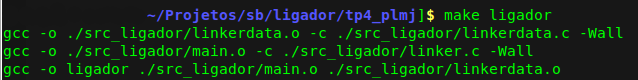
\includegraphics[scale=0.5]{./img/make.png}
 \caption{Comando Make}
\end{figure}

\begin{figure}[h!]
\centering
 
\includegraphics[scale=0.5]{./img/exec.png}
   \caption{Comando de execução do programa}
\end{figure}

\begin{figure}[h!]
\centering
 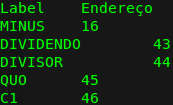
\includegraphics[scale=0.5]{./img/teste.png}
 \caption{saída usando verbose}
\end{figure}

\section{Conclusão}
\label{conclusao}
O trabalho correu sem grandes problemas, sendo a parte mais difícil a criação
dos progrmas de testes, pois montar alguns daqueles códigos em asembly é
extremamente difícil.

O programa atendeu a diversos valores de entrada e creio que a solução proposta
atenda ao especificado

\end{document}
